\documentclass{article}
\usepackage{latexsym}
\usepackage{amssymb,amsmath,amsfonts}
\usepackage{custom2}
\usepackage{graphicx} 
\usepackage{epstopdf} 
\usepackage{caption}
\usepackage{subcaption}
\usepackage{url}
\usepackage[all,arc]{xy}
\usepackage{enumerate}
\usepackage{mathrsfs}
\usepackage{booktabs}
\usepackage[pdftex]{hyperref}
\usepackage{lscape}
\usepackage{xcolor}
\usepackage{natbib}

\captionsetup{justification=RaggedRight, singlelinecheck=false}
\newcommand{\ra}[1]{\renewcommand{\arraystretch}{#1}}
\newcommand{\argmax}{\text{argmax}}
\newcommand{\Tr}{\text{Tr}}
\newtheorem{ass}{Assumption}

\addtolength{\evensidemargin}{-.5in}
\addtolength{\oddsidemargin}{-.5in}
\addtolength{\textwidth}{1.4in}
\addtolength{\textheight}{1.4in}
\addtolength{\topmargin}{-.5in}

\pagestyle{empty}

\title{Conflict and Strategy in Collective Computation}
\author{Eleanor Brush, David Krakauer, Jessica Flack}

\begin{document}
\maketitle

\section*{Abstract}
Collective computations occur in many biological systems, ranging in size from a brain made of billions of neurons to a social group made up of tens of monkeys. In each of these systems, a group-level output emerges from the behavior of individuals making decisions in noisy environments. In particular, in the brain and in primate social groups, pairs of individuals must make decisions about their relative relevance or ability. We use a leaky integrator model, a set of stochastic differential equations describing the dynamics of two decision variables, to model this decision process. The decisions made between each pair form a directed network over the whole group. The degree of consensus in the group about each individual's value, as determined by the decision network, is a collective computation that is informative about the individuals' true values. First, we show that the same model can be used to describe both neural and social systems. Next, we find that conflicts of interest in the decision process most strongly affect individuals at the bottom of the group and that conflicts of interest can incentivize these individuals to make more accurate decisions. Then, we find that when pairwise decisions are accurate, local properties of the decision network are the most informative, but global properties are more informative when decisions are less accurate or when the decision network is not fully formed. Finally, we find that the shape of the distribution of consensus scores is determined by the waiting costs of those decisions. 

\section*{Keywords }
collective computation, noisy learning, leaky integrator, decisions, social network, consensus, power

\section*{Introduction} 
Many biological systems perform collective computation.  A group of quorum sensing bacteria can sense its density and start to produce toxic, phosphorescent, or colorful molecules once the density is sufficiently high. Flocks of birds and schools of fish can stay together and navigate with beautiful coordinated motion. When presented with a set of moving dots, the brain, made up of billions of neurons, can decide whether more dots are moving left or right, even when the numerical superiority of one direction is very small. In social groups of primates, the distribution of the degree of consensus about each monkey's ability to use force is informative about the animals� abilities and the animals use estimates of this emergent property to decide how to behave. In each of these examples, the individual members of the group make decisions based on noisy environmental information and the collective computation emerges from those individual decisions. Through this two-step process the group produces a successful output or behavior, despite the computational limitations of its members and the conflicts of interest between them. While these examples come from quite different systems, the similarity in the phenomena suggest there may be common principles underlying collective computation in all of them. (In Table \ref{examples} we identify the components of the collective computation--- the environmental information, the individual, the decision that each individual must make, and the resulting collective computation---in each of these systems.)

%Both individuals involved in the decision value making a correct and fast decision. Since it takes time to gather enough evidence to make a correct decision, there is a tradeoff between accuracy and speed. Additionally, each individual might prefer that the decision be made in their favor, whether or not they truly have a higher ability.  This introduces a conflict of interest. Each individual will have a strategy to negotiate accuracy, speed, and their personal preferences.


To understand these collective computations, we must understand how the individuals make decisions. The sequential probability ratio test (SPRT) is the optimal way to decide between two alternatives in a noisy environment, in the sense that, for a given amount of time, the SPRT is the most accurate algorithm and, for a given error rate, the SPRT reaches a decision most quickly.  The algorithm works by keeping track of the amount of evidence supporting each alternative and deciding in favor of one once the evidence for it is sufficiently high. This algorithm assumes the individuals making the decision have perfect memory, but in reality this is rarely the case.  A simple way to model memory loss is to assume that the amount of evidence decays back toward zero at each point in time. This forgetful model of decision-making can be transformed into a leaky integrator model, a set of stochastic differential equations (SDEs) describing how the variables accumulating evidence for each alternative change over time. The random walk described by the SDEs is biased by the true state of the environment. This model is applicable to any system in which an individual with imperfect memory gathers evidence and chooses the alternative for which it has gathered more support.  

The leaky integrator model has been applied to neural decision-making, and it successfully predicts performance in a number of experiments  \citep{Eckhoff:2008uq, Brown:2005fk,Feng:2009kl,Bogacz:2006uq}. In this system, each of two neural populations responds to evidence for either left or right motion.  The SDEs describe how the firing rates of the two populations change over time and a decision is made once one the difference in firing rates is sufficiently high. The visual stimulus driving this decision process is usually a set of dots, some percentage of which are moving coherently either left or right and the rest of which are moving randomly.  The bias in the SDEs is in favor of the direction in which the coherent dots are moving.  The model could also describe neural populations deciding between other possibilities, for example between up and down motion or between two colors. In order to distinguish between or rank a whole set of possibilities, the brain could rely on a group of neural populations, each responding to one of the options. 

While the SPRT has been applied to animal conflicts  \citep{Froment:2010fk}, to our knowledge the leaky integrator model has not been. In this application, each of two animals has an opinion about its dominance with respect to the other, which goes up or down as the animal wins or loses fights against its opponent. Even if one animal is stronger, the outcome of a fight is affected by the identity and presence of each animal's allies, their motivation levels,  external environmental variables, and other stochastic factors, which introduce noise that is captured by the SDEs.   The bias in the model is in favor of the animal that is more likely to win. Once an animal's opinion goes below a threshold, it decides to agree to be subordinate to the other. A correct decision is one in which the weaker individual makes this agreement.  In pigtailed macaques ({\it Macaca nemestrina}), there is a formal subordination signal that an animal can use to communicate its agreement to the subordinate role in their relationship \citep{Flack:2007kx, Flack:2006fk,Flack:2004oq, Waal:1985fk,Caldecott:1986uk,Preuschoft:2004ly}.  This signal marks the end of the decision process.

In both systems, the decisions between pairs of individuals form a directed network, each edge of which reflects a decision about the relative values of the nodes it connects. In many systems, the degree of consensus in a group about each individual's value is informative about the individuals'  true values and affects the individuals' functional behaviors \cite{Brush:2013fk}. In previous work, we developed a number of network metrics to measure the degree of consensus in a group about each individual and we identified a set of algorithms that produced scores that were predictive of individuals' functions in a group in multiple empirical systems \cite{Brush:2013fk,Flack:2006uq}. The consensus scores that result from applying one of these consensus measures to the decision network is the collective computation that we are interested in. There are three factors affecting this collective computation: the statistical properties of the environment, the strategies individuals use to make decisions about their relative values, and the method of measuring consensus from a network of decisions.  

In the social system, this consensus is referred to as social power. In macaques, power is a useful variable since it reflects the animals' true fighting abilities and the animals themselves use estimates of their peers' and their own power to decide how to behave \cite{Flack:2004oq,Flack:2006fk,Flack:2006uq}.  The distribution of power scores in a group of pigtailed macaques is heavy tailed and this allows the individuals in the tail to perform different functions  than the rest of the animals \cite{Flack:2005uq,Flack:2006fk,Flack:2006uq}.  The shape of the power distribution varies across species of macaques \cite{Caldecott:1986uk,Flack:2004oq,Preuschoft:2004ly,Waal:1985fk,Thierry:2000ij}, and it is an open question whether this variation can be explained by differences in the underlying distributions of fighting abilities, by differences in the way animals in different species resolve their differences, or by other mechanisms. Consensus may be important in neural systems, as well.  A number of neural populations may respond to or encode different environmental stimuli or variables.  The consensus in a group of neural populations about the value of a number of environmental stimuli could help the brain make decisions about the relative values of many possibilities. 

In this paper, we derive the leaky integrator model from a simple mechanistic description of the accumulation of information, making two simplifying assumptions about the timescales on which probabilistic events occur \cite{Gillespie:2000fk}. While the model has been successfully used to describe neural learning dynamics, its application has been rather phenomenological and this mechanistic derivation justifies its application in any system where the assumptions are reasonable. We then use the leaky integrator model to answer the following questions. Do differences in the decision making model as it is applied to neural and social systems affect the accuracy of the decision process? What strategies should individuals with conflicting interests use to make decisions in a group context? How do the individuals' strategies affect the collective computation? What function of the decision network produces the most informative collective computation? How well does our model describe empirical social systems?

\section*{Model} 
\subsection*{Stochastic differential equations }    
\ In chemical systems, stochastic differential equations are used to describe the dynamics of the concentrations of various solutes, and these Langevin equations can be derived from a mechanistic description of chemical reactions \cite{Gillespie:1992vn,Gillespie:2000fk}. However, the SDEs used to model noisy decision processes are usually applied without any mechanistic justification. By following the mathematical derivation of the SDEs in chemical systems given by Gillespie \cite{Gillespie:2000fk},  we can derive the SDEs used in the leaky integrator model.

In a decision between two alternatives, there are two decision variables, $X_1$ and $X_2$, each indicating the evidence accumulated for one of the options.  In the absence of any input, the decision variables leak back towards $0$ with rate $\ell$.  (A table of all variables used in the text is given in Table \ref{variables}.)  If there is no input, then over a period length $\tau$ a decision variable decreases as $X(t+\tau)=(1-\ell\tau)X(t)$. If there is input, each decision variable will incorporate the new evidence by responding positively to one type of input and negatively to the other.  Specifically, $X_1$ increases by an amount $b$ when it sees evidence for option $1$ and decrements by $-b$ when it sees evidence for option $2$, and conversely for $X_2$.  In the neural case, one neural population responds positively to left dots and negatively to right dots and the other neural population does the opposite.  In the social case, one animal's estimate of its own dominance increases when it wins fights and decreases when it loses fights, and the other animal's estimate does the opposite.  For clarity, in the following we will refer to the inputs as left or right dots, but they could also be referred to as wins or losses. To calculate the variables at time $t+\tau$, we  count how many times each of type of input occurred in the time since $t$ and add the changes resulting from these events to the background leaky estimate (as in \cite{Gillespie:2000fk}):
\begin{align*}
X_1(t+\tau)&=(1-\ell\tau)X_1(t)+b\times\# \text{ of left dots in }[t,t+\tau)-b\times\# \text{ of right dots in }[t,t+\tau)
\\ X_2(t+\tau)&=(1-\ell\tau)X_2(t)-b\times\# \text{ of left dots in }[t,t+\tau)+b\times\# \text{ of right dots in }[t,t+\tau). 
\end{align*}

Our first assumption is that the rates at which the two types of inputs occur is constant over time.  We can thus describe the number of each type of event with a Poisson random variable, $N_\text{L}$ and $N_\text{R}$, giving 
\begin{align*}
X_1(t+\tau)&=(1-\ell\tau)X_1(t)+bN_\text{L}-bN_\text{R}
\\ X_1(t+\tau)&=(1-\ell\tau)X_2(t)-bN_\text{L}+bN_\text{R}.
\end{align*}
If events happen at a rate $r$ and the event is a left dot with probability $c$ and a right dot with probability $1-c$, then the expectation of $N_L$ and $N_R$ in a period of length $\tau$ are, respectively, $\tau r c$ and $\tau r(1-c)$. In the neural case, $c$ is related to the ``coherence'' of the visual stimulus.  A value of $c$ close to $0$ or $1$ means that most of the events are of one type or the other and the decision is easier to make than when $c$ is close to $.5$.

If enough events happen in the period of time from $t$ to $t+\tau$ then we can approximate the Poisson random variables with normal random variables with mean and variance equal to the mean of the Poisson random variables.  Our second assumption, then, is that the period of time of length $\tau$ is long enough to make this approximation. Let $Z_\text{L}$ and $Z_\text{R}$, be independent standard Normal random variables, i.e. with mean $0$ and standard deviation $1$, giving
\begin{align*}
X_1(t+\tau)&=(1-\ell\tau)X_1(t)+b\bigg(\tau rc+\sqrt{\tau rc}Z_{\text{L}}\bigg)-b\bigg(\tau r(1-c)+\sqrt{\tau r(1-c)}Z_{\text{R}}\bigg)
\\X_2(t+\tau)&=(1-\ell\tau)X_2(t)-b\bigg(\tau rc+\sqrt{\tau rc}Z_{\text{L}}\bigg)+b\bigg(\tau r(1-c)+\sqrt{\tau r(1-c)}Z_{\text{R}}\bigg).
\end{align*}
Finally, as we make the period of time shorter and shorter, making $\tau$ infinitesimally small, these equations become stochastic differential equations,
\begin{equation}
\begin{array}{ll}
dX_1&=\bigg(-\ell X_1(t)+br(2c-1)\bigg)dt+\bigg(b\sqrt{rc}\bigg)dW_\text{L}t-\bigg(b\sqrt{r(1-c)}\bigg)dW_\text{R}t
\\dX_2&=\bigg(-\ell X_2(t)-br(2c-1)\bigg)dt-\bigg(b\sqrt{rc}\bigg)dW_\text{L}t+\bigg(b\sqrt{r(1-c)}\bigg)dW_\text{R}t
\end{array}
\end{equation}
where $dW_{\text{L}}$ and $dW_{\text{R}}$ are independent Brownian motions representing, respectively, the left and right inputs.  The assumptions about the timescales on which inputs occur are reasonable in the social system, and the successful application of this type of model to neural populations implies they are not unreasonable in that system.  In Table \ref{variables}, we list the inputs, outputs, and variables of the decision model and how they should be interpreted in the neural and social systems.


\subsection*{Reaching a decision }\ There are two ways to use the decision variables $X_1$ and $X_2$ to make a decision.  If the difference in the variables can be observed, it indicates the relative strengths of the evidence for each option. If $Y=X_1-X_2$, the system should decides on $X_1$ when $Y$ is large and positive and on $X_2$ when $Y$ is large and negative.  Specifically, there are two thresholds, $T_1$ and $T_2$ such that if $Y>T_1$ the decision is for $X_1$ and if $Y<-T_2$ the decision is for $X_2$.  However, it may be the case that the difference in the variables cannot be observed.  In this case, the decision depends on whether $X_1$ or $X_2$ hits a threshold first.  Again, there are two thresholds, $T_1$ and $T_2$, and if $X_2<-T_2$ the decision is for $X_1$ and if the $X_1<-T_1$ the decision is for $X_2$. 

In the neural system, the two stochastic equations describing the activity of the two neural populations integrating environmental evidence are often reduced to the one-dimensional equation describing the difference in the activity levels \cite{Brown:2005fk,Bogacz:2006uq,Feng:2009kl}.  The reduced model is easier to analyze, but there is no empirical evidence for a mechanism in the brain that measures the difference in activity rates and the full two-dimensional model should apply equally well to neural decision making, a possibility we consider here. In the social system, we cannot make any assumptions about the existence of a third party evaluating the difference in the opinions of the two animals.  A decision, i.e. the emission of a signal from one of the two animals, is only reached when one of the two animals' opinions goes below its threshold.  The social system is therefore inherently two-dimensional.  In Table \ref{differences}, we compare how the decision is made and how the decision process is optimized in the two systems.

\subsection*{Utility of the decision }
\ The thresholds affect how long the decision takes and the probabilities with which each output is decided upon.  A good decision is one that reaches the correct output quickly, i.e.\ the expected time until a decision is reached (decision time, DT) and the probability that an incorrect decision is made (error rate, ER) are low.   However, it is impossible to minimize both simultaneously since waiting longer and accumulating more evidence makes the decision more accurate and conversely.  It may also be the case that each individual prefers one output over the other, regardless of which is correct.  In the social case, each animal would prefer that its partner agree to be subordinate, whether or not it is truly stronger.  In the neural case, different neural populations may receive different rewards if the decision reaches different outcomes, regardless of which of the alternatives is correct.  Therefore, an individual may want to maximize the probability that its preferred outcome is reached (probability of preference being chosen, $\text{PP}_i$).    

To describe the tradeoffs between error rate, decision time, and preference, we quantify the utility of the decision process by introducing three weights, $w_1$, $w_2$, and $w_3$ such that $w_1+w_2+w_3=1$.  These weights describe how the three quantities are prioritized.  For individual $i$, we define
\begin{equation*}
U_{i}=w_1\text{ER}+w_2\text{DT}+w_3(1-\text{PP}_i).
\end{equation*}
The decision is better if $U_i$ is lower.  In the social system, $w_2$ can be interpreted as the cost of fighting since when $w_2$ is higher, the time spent fighting until a decision is reached is more costly.  In the neural system, $w_2$ depends on whatever costs the brain or the whole animal incurs by waiting for a decision. Given that $\text{PP}_1=1-\text{PP}_2$, it is impossible for them both to maximize $\text{PP}_i$, so the personal preference weight $w_3$ indicates the strength of the conflict of interests between individuals and how stubborn the individuals are about their preferences. In the social system, $w_3$ can be interpreted as the benefit from being the dominant animal in a pair.

As show in the Supplementary Information, each of the three decision properties, ER, DT, and PP satisfies a partial differential equation that depends on the SDEs and the parameters of the model. There are analytical solutions to these equations when the system of SDEs is reduced to one dimension. However, we were not able to find an analytical solution for the full two-dimensional system and we therefore used numerical methods to solve the PDEs in this case.

\subsection*{Nash equilibrium thresholds }
\ In a group of individuals, each with a value $a_i$, the difficulty with which the pair $i,j$ makes a decision increases with the difference in value, i.e. $c_{ij}$ is an increasing function of $|a_i-a_j|$. In the social system, the value $a_i$ reflects an animal's fighting ability. In the neural system, the value $a_i$ is high if the property (e.g.\ left movement or red color) a neural population responds to is abundant in the visual stimulus. We assume that each individual has the same decision threshold for all the decisions processes with each of its peers and, given those thresholds, each individual $i$ has a utility $U_{ij}$ from its decision process with individual $j$ and a total utility given by the average of these, $\langle U_{ij}\rangle _j$. For each set of values $\{a_1,\dots,a_N\}$, we find the Nash equilibrium thresholds such that no individual has an incentive to choose another threshold to improve its utility.  Since the Nash thresholds depend on the values $\{a_1,\dots,a_N\}$,  we repeatedly draw a set of values from a uniform distribution and find the Nash thresholds for each set. Then we find the average Nash threshold as a function of an animal's rank in the set of fighting abilities.    

\subsection*{Collective computation }
\ For each set of values $\{a_1,\dots,a_N\}$ and Nash thresholds $\{T_1,\dots,T_N\}$, we find the probability that each pair will reach either outcome and the expected time it will take.  We use these probabilities to generate a set of decisions between all pairs.  We use the convention that a decision is sent from $i$ to $j$ if $j$'s preference prevailed.  To incorporate the time it takes for a decision to be reached and allow for multiple decisions to be made, at each point in time $t$, we define the weight of the edge from $i$ to $j$ to be
$$
\begin{array}{lllll}
0 & \text{ if the decision was made in favor of } i\text{ or } DT_{ij}>t 
\\t-DT_{ij} & \text{ if the decision was made in favor of } j\text{ and } DT_{ij}>t 
\end{array}
$$
Once $t$ is greater than the maximum decision time between all pairs of individuals, all edges of the network will have formed.

Given a decision network, there are many ways to measure the consensus present in the group about each individual's value \cite{Brush:2013fk, Flack:2006uq}. These formalisms assign a consensus score to each node in the network.  In the following we consider four  consensus formalisms.  The first and simplest is simply the unweighted in-degree of a node, i.e. the number of individuals deciding in favor of each individual.  The second is the weighted in-degree of a node, which is a finer measure than the unweighted in-degree since it takes into consideration the strength of each decision made in favor of the node.  The third is the entropy of the distribution of the number of decisions made in favor of each individual, which gives a coarse measurement of how uniformly all other individuals in the group behave with respect to a focal individual.  The fourth is the eigenvector centrality of the decision network, which measures how central each node is in the global structure of the network.  For more details see \cite{Brush:2013fk}. Using many random sets of fighting abilities, we find the mutual information between the consensus scores from the network at each time $t$ and the true values, for each consensus formalism. We also find the average skewness of the set of consensus scores.

\section*{Results}
\subsection*{Decision making is as accurate without a third party arbiter. }
\ First we compare the decision making process in the full two-dimensional system and in a reduced one-dimensional system to see whether decisions are made more accurately or quickly in one or the other.  To make the systems directly comparable, we assume in both cases that the thresholds are symmetric, i.e. $T_1=T_2$.  We find that the two-dimensional process is as accurate as the one-dimensional process.  That is, for a given expected time to reach a decision, the two-dimensional process will reach the correct decision with the same probability (Supplemental Figure \ref{dimensionality}). Because they perform equally well and because the two-dimensional system is more appropriate for the social system (and perhaps the neural system as well), we use the two-dimensional system in the rest of our analyses. While the results come from an analysis of the two-dimensional system, they should also apply to the reduced system.
%Accuracy decreases as leak rates ($\ell$) become higher, but increases when the strength of the input ($c$) is higher.

\subsection*{A conflict of interests incentivizes individuals in the bottom of the group to make more accurate decisions. }
\ We start with a pair of individuals, i.e. a group of size two, to build intuition for how the optimization weights affect the Nash equilibrium thresholds.  If accuracy of the decision is the only thing that matters ($w_1=1$), the weaker individual will set his threshold as low as possible and the stronger animal will set his threshold as high as possible, since the decision is correct when the weaker animal gives up first. When only personal preference matters and there is a strong conflict of interest between the individuals($w_3=1)$, both will set their threshold high since there is no incentive for the individuals to stop accumulating evidence. As the importance of decision time increases (i.e. waiting costs increase), both individuals will lower their thresholds in order to reach the decision more quickly, whatever that decision may be (Figure \ref{nasheq}). The accuracy with which a pair using Nash thresholds can reach a decision is highest when only error rate matters ($w_1=1$) and decreases as either decision time or personal preference become important (Figure \ref{nasheq}).  

In a group with more than two individuals, an individual's position in the group affects how it makes the tradeoff between error rate, preference and decision time.  As in a pair, prioritizing accuracy tends to lead individuals with high value to set high thresholds and those with low values to set low thresholds and prioritizing personal preferences tends to lead all individuals to set high thresholds (Figure \ref{groupeq}). The difference in an individual's threshold between when accuracy is important and when personal preferences are important is largest for the individuals at the bottom of the group. Individuals at the top of the group will set high thresholds in either case. Individuals toward the bottom, however, will set lower thresholds when they prioritize accuracy then when they prioritize personal preferences. This is because choosing a higher threshold increases waiting time in decisions with respect to all individuals, decreases the accuracy of its decisions with respect to higher animals, and only slightly increases the accuracy of its decisions with respect to other low individuals. In other words, individuals at the bottom of the group sacrifice some accuracy in their decisions with respect to each other in order to decrease their overall decision times. This leads to the counterintuitive result that making personal preferences more important (i.e. having a larger conflict of interest) and making accuracy less important actually increases the average accuracy of the decisions made between individuals at the bottom of the group.

This in turn leads to a very slight increase in the average accuracy of all pairs in the group (Figure \ref{groupeq}).  Therefore, in a group with more than two members, increasing the importance of decision time decreases the average accuracy, but increasing the strength of conflicts of interest leads to a (slight) increase in accuracy. While the improvement is small, it is very different from the decrease in accuracy caused by increasing the strength of conflicts of interest in a pair. For every measure of consensus, the mutual information between the consensus scores and the true values increases with average pairwise accuracy.  Thus, the information content of the consensus scores is also maintained when the individuals prioritize personal preference rather than error rate. We show in Supplemental Figure \ref{groupsize} that the size of the group does not affect the accuracy with which the group, the top quartile of the group, or the bottom quartile of the group makes decisions.

\subsection*{Eigenvector centrality provides the most information when accuracy is high but imperfect and when the network is developing. }
\ First, we consider the mutual information between the consensus formalisms applied to a fully formed decision network and the true values. For each of the four measures we consider, there are combinations of  the optimization weights that make it the most informative formalism (Figure \ref{bestmetric}). When waiting costs are low, the finer measures of consensus--- weighted in-degree and eigenvector centrality---outperform the coarser measures---in-degree and entropy---because in these circumstances, the edges of the decision network tend to be accurate and the finer measures make use of more information from the network and make finer distinctions. When there are no waiting costs and personal preferences are important, all individuals have high thresholds,  weighted in-degree outperforms eigenvector centrality (Figure \ref{bestmetric}).  
%%WHY?!?!?
%This makes sense since when each edge in the decision network accurately reflects the difference in value between individuals, weighted in-degree received is informative about an individual's position in the group.  In particular, weighted in-degree out performs eigenvector centrality by correctly resolving small differences between the highest value individuals. 
When the pairwise decisions are less accurate, global structure of the decision network provides information about values that the individual relationships do not, so eigenvector centrality is the the most informative about the individuals' true values (Figure \ref{bestmetric}).  When accuracy is quite low, weighted in-degree and eigenvector centrality correctly rank the very highest individuals, but cannot distinguish between the lower half of the group. On the other hand, in-degree assigns the same scores to the few highest individuals, but correctly resolves the differences between the bottom half, making it slightly more informative over all. When accuracy is very low, none of the measures are very informative, but entropy correctly gives the very lowest individuals low scores and the very highest individuals high scores, giving it an edge over the other measures.

The information content of the different formalisms show different patterns as the network is forming (Figure \ref{bestmetric}). The information content of all formalisms show an initial rise as edges start to form in the decision network. When there are waiting costs and hence some inaccurate edges in the network, as these edges develop, there is a decrease in the information content of the three local measures---weighted in-degree, in-degree, and entropy---but not in eigenvector centrality. As the network becomes more fully developed, the information content of the three local measures recovers, in some cases even surpassing the information content of eigenvector centrality. Therefore, regardless of which measure is most informative on a fully developed network, as long as there are non-zero waiting costs, eigenvector centrality has the advantage of never losing information content as edges are added to the network and consistently performing well on networks that are not fully formed.




\subsection*{The skewness of the power distribution is maximized when decisions are moderately accurate. }
\ For each measure of consensus in the decision network, we find the average skewness of the distribution of consensus scores of a group using Nash thresholds, as they depend on optimization weight.  We find that, for all measures, skewness is maximized at intermediate waiting costs and does not depend strongly on the tradeoff between error rate and preference (Figure \ref{skewness}). (Results for number of signalers are shown in Figure \ref{skewness} and others are similar).  When waiting costs are low and accuracy is high, the decisions accurately represent the individuals' true  abilities, so the distribution of number of signalers accurately represents the distribution of abilities, which is not very right-skewed.  When waiting costs are high and accuracy is low, decisions are so noisy that all individuals receive a similar number of decisions, giving a distribution that is quite uniform and not right-skewed.  At intermediate waiting costs, the decisions between individuals with low to middle abilities are very noisy, so that the individuals in the bottom and middle of the group receive a similar number of signals, but all individuals make accurate decisions with the top few individuals, which gives them high scores and results in a right-skewed distribution.


\subsection*{Decisions in a group take longest between individuals with similarly high abilities. }
\ When waiting costs are low, the pairs that take the longest to reach a decision are those with similar fighting abilities, but pairs with different abilities also take a fairly long time.  When waiting costs are high, all pairs reach decisions quickly.  At intermediate costs, most pairs can reach a decision quite quickly, except those who have similar and high abilities (Figure \ref{groupeq}).  Pairs with similar and high abilities always take as long or longer to make a decision than any other pairs do.
 

\section*{Discussion}

From a mechanistic description of a decision-making process, we derive a set of stochastic differential equations that describe how two individuals accumulate evidence from a noisy environment.  The model can be equally well applied to the firing rates of neural populations observing a visual stimulus and the beliefs of two monkeys about their relative dominance based on their fighting history.   Either the absolute value of the decision variables or the difference in their values can determine the outcome of the decision.  We find that, for a given decision time, the accuracy of the decision does not depend on which of these mechanisms is used.  In order for the difference in variables to be used, a third party arbiter needs to be present to evaluate the value of each decision variable and find their difference.  In the brain, it might be the case that there is a third neural population whose activity depends on the two populations gathering external evidence. In a social group, there is no third party gathering information about the opinions of two monkeys in order to dictate when the decision establishing their subordination-dominance relationship should be made.  The fact that the existence of this third party arbiter does not affect the model output highlights the similarity between the two systems and it means that the results of a model without the arbiter apply in either case.

Individuals in biological systems are likely to be selfish and stubborn, both in order to maximize their own welfare and because prioritizing accuracy requires knowing which the right answer is beforehand.  One might expect that individuals valuing their preference at the expense of the accuracy would tend to make decisions that were less accurate.  In a pair, this holds true.  However, when there is a group of individuals all making this tradeoff, valuing preferences over accuracy improves the accuracy with which individuals in the bottom of the group resolve their differences. This slightly increases the average accuracy of the whole group, which translates into a slightly more informative collective computation.  While the increase in accuracy is not very big, it is encouraging that, as long as there are non-zero waiting costs, conflicts of interest do not undermine the group's ability to perform a collective computation. In every biological system, there are constraints on the amount of time an individual can take to make a decision so the condition of non-zero waiting costs is likely to be satisfied.

Usually, only two neural populations are included in models of neural decision making (although see XXX).  Further, it is usually assumed that neural populations in the brain value accuracy, since the whole organism receives a benefit from making a correct decision in a short time.  But it is possible that different neural populations receive different rewards from making different decisions, regardless of which decision is the correct one.  Only by considering a group with more than two members do we find the surprising result that the accuracy of a collective computation can be improved by introducing conflicting interests.  This might suggest that in situations where a group of neural populations are recruited to make a decision, we could expect to find that they have different preferences, rather than all valuing accuracy. Our result also has  implications for designing networks with which to make computations.

There are many different ways of measuring the consensus about individuals' values from a decision network \cite{Brush:2013fk,Flack:2006uq}. Each network metric represents a different way of performing a collective computation. We find that when the accuracy of pairwise decisions high, finer measures like weighted in-degree and eigenvector centrality are the most informative about the true states of the nodes, but  when pairwise accuracy is quite low, coarser measures like in-degree and entropy perform best. We also find that eigenvector centrality performs well on network that are not fully formed. As network scientists, if we are presented with an interaction network, we would like to know how to measure the consensus present in the network about each node.  If we have a sense of the accuracy with which the edges reflect true differences in the states of the nodes or how complete the network is, these results give a rule of thumb for how to pick a measure of consensus. Since eigenvector centrality always performs optimally or close to optimally on a fully formed network and it performs optimally on a network that is still forming, eigenvector centrality seems to be generally a good algorithm to use. 

As members of a social group about which they would like to have information, the monkeys may use these measures (or approximations of them) to estimate their own and their peers' abilities. In previous work, we found that both eigenvector centrality and weighted in-degree (and variants thereof)  produced scores that were informative about animals' functional behavior in a group of pigtailed macaques.  This may be tell us something about the optimization weights the animals in that group are using.  If so, it would suggest that decision time is less important than a combination of error rate and the probability of being dominant. It also suggests that if animals in different species prioritize fighting costs and the benefits from being dominant differently, we might expect to find that those animals use different properties of their social networks to estimate the power structure of the group.  

The skewness of the power structure that results from this collective computation in social groups of macaques has important functional consequences \cite{Flack:2004oq,Flack:2006fk}. We find that for most measures of power the skewness of the distribution of power scores is maximized at intermediate waiting costs.  In our data, we observe a right-skewed distribution of power \cite{Brush:2013fk,Flack:2006uq}.  To the extent that our model recapitulates the empirical system, this would suggest that waiting costs are neither the only priority nor are they ignored completely.

Different species of macaque have stereotypical power structures with different amounts of skewness \cite{Flack:2004oq,Preuschoft:2004ly,Waal:1985fk}.  One explanation might be that the distribution of fighting abilities is different from species to species, for instance if there is more or less variation in body size.  However, our model suggests that even if the underlying distribution of fighting abilities are identical, the priorities given to preference, error rate, and waiting costs can affect the distribution of power.  The benefit of having a partner agree to be subordinate, the benefit of reaching the ``correct" agreement, and the costs of fighting may vary from species to species, causing variation in the shape of the power structure.

Individual-based models and computer simulations have previous been used to explain the social structures of macaques \cite{Hemelrijk:2011fk,Hausfater:1981fk}. In a more complicated model, the ``aggressiveness'' of animals moving in a spatially explicit area affected the shape of the dominance hierarchy \cite{Hemelrijk:2011fk}.  While the mechanisms of that model are quite different, ``aggressiveness'' could be argued to be similar to disregarding fighting costs and prioritizing preference.  Neither the authors of that work nor we found that a difference in the underlying distribution of fighting abilities is required to change the distribution of dominance or power.  In other words, in both models, the collective computation that results in a power structure depends more on how the individuals interact and collect information than on the distribution of fighting abilities. 

It is difficult to assess whether decisions in empirical systems are being made accurately, but it is easier to measure how long they take.  In a group, each pair of individuals experiences the difference in their abilities, but their absolute positions within the group also matter.  In data from a captive population of macaques, we observe that pairs of animals with high abilities reach agreements about their relative dominance but that pairs of animals with low abilities sometimes do not reach such agreements (Flack, unpublished data).  In our model, decisions between pairs who have similar and high abilities always  take as long or longer than decisions between any other pairs.  This discrepancy indicates that our simple model is missing a level of social complexity that could explain this empirical pattern.  

There are (at least) two modifications to the model that we expect would produce results closer to the empirical observations.  First, in the model, the rates at which animals fight each other do not depend on the abilities of the animals.  However, it is likely that animals with lower abilities are less mobile and encounter their peers at a lower rate than animals with higher abilities who are more free to range throughout the group.  In the model, this heterogeneity in encounter rate would make the decisions between animals with low encounter rates take longer.  Second, in the model, all animals value preference, error rate, and waiting costs equally.  However, it is likely that the benefits from receiving a subordination signal from a partner and the costs of fighting depend on both animals' abilities.  If animals with low ability  do not value an agreement with other animals with similar abilities, there would be less incentive for them to reach an agreement.  These types of heterogeneity would make our model more biologically realistic when applied to the social system, but without them it is general enough to be applied to a number of systems in which collective computations are being performed.  

We assumed that the individuals in a group use Nash equilibrium thresholds, but in order to do so, they would first have to determine what those are.  By assuming that they use these optimal strategies, we are able to analyze the consequences of what it means to be ``optimal," but it neglects the interesting question of how those optimal strategies might be reached. Another way to make our model more realistic would be to include a way for the individuals to learn what thresholds to use. Finding the appropriate timescale separation between the dynamics of how strategies are learned and the decision dynamics and the consequences of this additional level of learning are left for future work.

We apply a noisy learning model to two different biological systems, one neural and one social, and our model reduces to previously studied ``war of attrition'' games in the game theory literature when the abilities of the two individuals are equal.  The similarities between these three frameworks---neural decision making, social decision making, and game theory---suggest that there are common principles of decision making through conflict that are applicable to a number of systems. Conflict and strategy are not usually ascribed to the neural model, and the war of attrition is not usually thought of as a process through which the pair of competitors reaches a decision about an external truth.  Our work is a first step toward unifying these different frameworks and better understanding the importance of conflict and strategy in collective computation.
%%other applications?

\section*{Acknowledgements }
This publication was made possible through the support of a subaward from the Santa Fe Institute under a grant from the John Templeton Foundation for the study of complexity. The opinions expressed in this publication are those of the author(s) and do not necessarily reflect the views of the John Templeton Foundation. EB acknowledges support from the training grant NIH 5T32HG003284.


\section*{Figures}

\begin{figure}[ht]
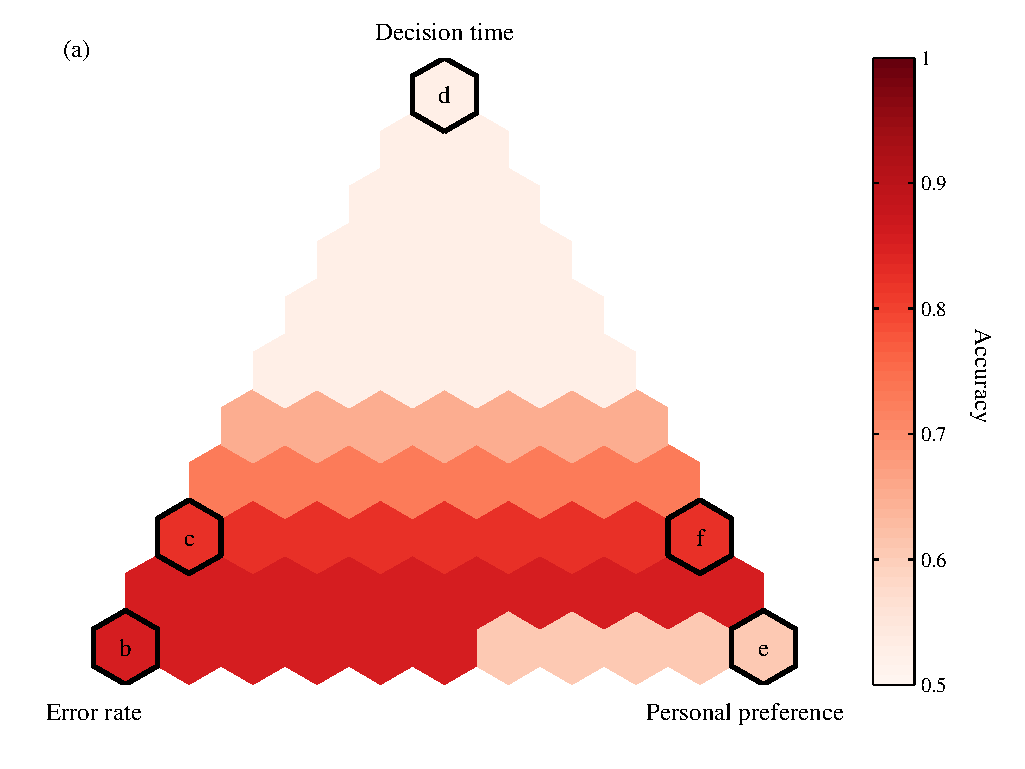
\includegraphics[]{pairwiseaccuracy.pdf}
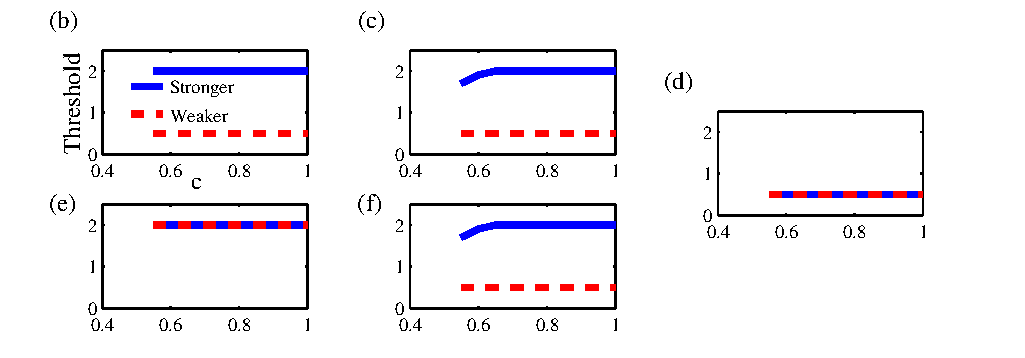
\includegraphics[]{nasheq_thresholds.pdf}
\caption{\label{nasheq} The accuracy of a pair using Nash equilibrium thresholds decreases as the weight given to decision time increases.  (a) In the upper panel, the color indicates the accuracy of a decision made by a pair making a difficult decision ($c=.55$) using Nash equilibrium thresholds, as a function of the optimization weights, $w_1$, $w_2$, $w_3$.  In the lower left corner of the simplex, only error rate matters ($w_1=1$).  In the upper corner, only decision time matters ($w_2=1$).  In the lower right corner, only preference matters ($w_3=1$). Accuracy decreases as $w_2$ increases but is not greatly affected by a tradeoff between $w_1$ and $w_3$. In (b)-(g) we show how the Nash equilibrium thresholds depend on the difficulty of the decision ($c$). The optimization weights for each panel are indicated in the simplex with the corresponding letter. Parameters: $w_1=1$, $w_2=0$, $w_3=0$ (b), $w_1=0.8$, $w_2=0.2$, $w_3=0$ (c), $w_1=0$, $w_2=1$, $w_3=0$ (d), $w_1=0$, $w_2=0$, $w_3=1$ (e), $w_1=0$, $w_2=0.2$, $w_3=0.8$ (f), $b=1$, $r=1$, $\ell=0.1$. }
\end{figure}

\begin{figure}[ht]
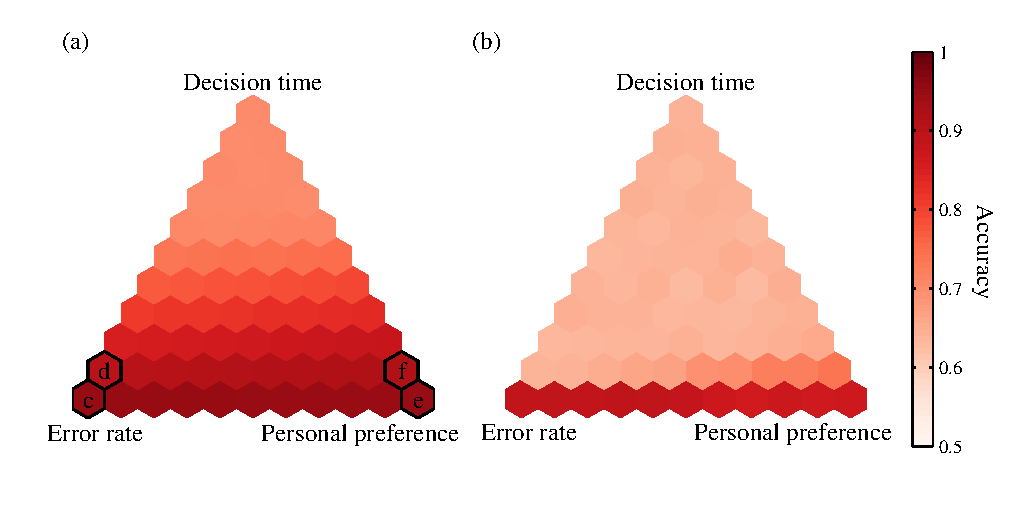
\includegraphics[width=\textwidth]{groupaccuracy.pdf}
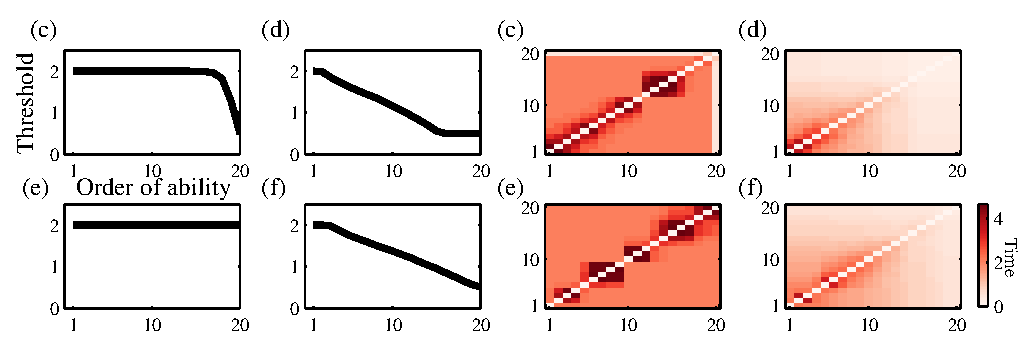
\includegraphics[width=\textwidth]{groupeq_thresholds.pdf}
\caption{\label{groupeq}   The accuracy of a group using Nash thresholds decreases as the weight given to decision time increases.  In the upper panels, the color indicates (a) the average accuracy of the whole group and (b) the average accuracy of the decisions between individuals in the bottom quartile using Nash thresholds, as a function of the optimization weights, $w_1$, $w_2$, $w_3$.  In the lower left corner of the simplex, only error rate matters ($w_1=1$).  In the upper corner, only decision time matters ($w_2=1$).  In the lower right corner, only preference matters ($w_3=1$). Both bottom-quartile and total accuracy decrease as $w_2$ increases, and the increase in bottom-quartile accuracy as $w_3$ increases drives a slight increase in total accuracy.  In (c)-(f) we show how the group-context Nash thresholds (left panels) and decision time for each pair (right panels) depends on the true order of value where $1$ is the strongest individual and $20$ is the weakest. The optimization weights for each panel are indicated in the simplex with the corresponding letter.  For low waiting costs (c and e), it takes longest for pairs with similar values to reach a decision.  For slightly higher waiting costs (d and f), it takes longer for pairs with similar and high values to reach a decision. Parameters: $w_1=1$, $w_2=0$, $w_3=0$ (c), $w_1=0.9$, $w_2=0.1$, $w_3=0$ (d), $w_1=0$, $w_2=0$, $w_3=1$ (e), $w_1=0$, $w_2=0.1$, $w_3=0.9$ (f), $N=20$, $b=1$, $r=1$, $\ell=0.1$. }

\end{figure}


\begin{figure}[ht]
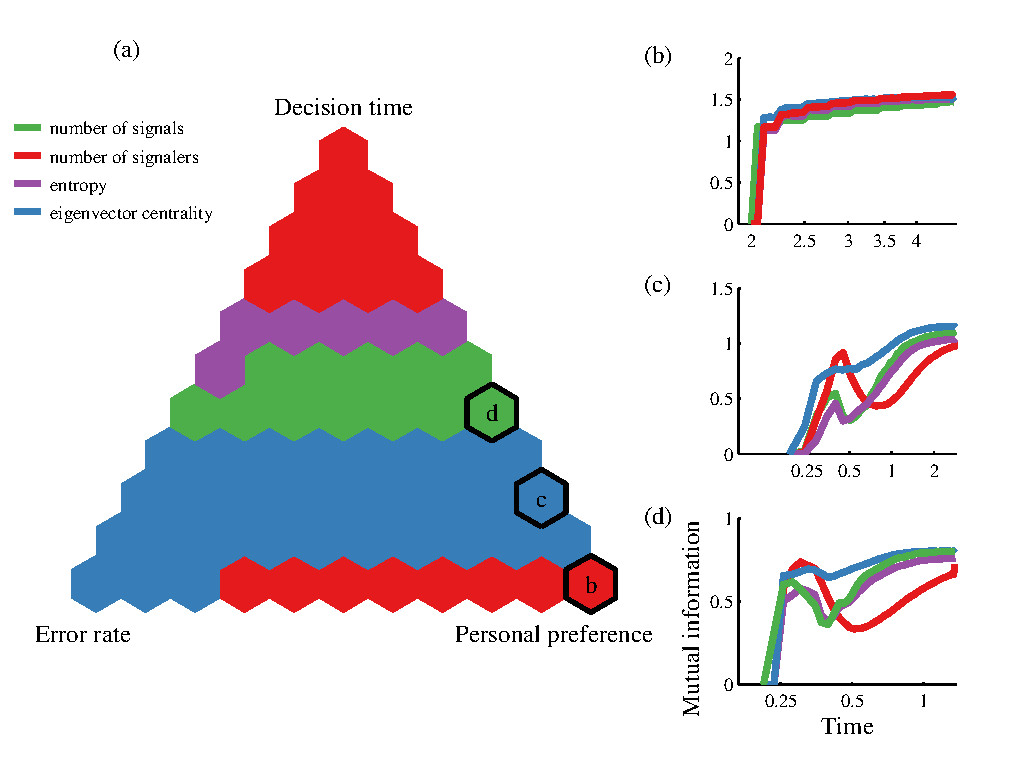
\includegraphics[width=\textwidth]{info.pdf}
\caption{\label{bestmetric} The best method to use for measuring consensus in the decision network depends on how accurate decisions are on average.  (a) In the left panel, the color indicates the most informative consensus formalisms. In the lower left corner of the simplex, only error rate matters ($w_1=1$).  In the upper corner, only decision time matters ($w_2=1$).  In the lower right corner, only preference matters ($w_3=1$). In (b)-(d) we show how the mutual information of each consensus formalisms increases over time. The optimization weights for each panels are indicated in the simplex with the corresponding letter. Parameters: $w_1=0$, $w_2=0$, $w_3=1$ (c), $w_1=0$, $w_2=0.2$, $w_3=0.8$ (d), $w_1=0$, $w_2=0.4$, $w_3=0.6$ (e),  $N=20$, $b=1$, $r=1$, $\ell=0.1$.}
\end{figure}


\begin{figure}[ht]
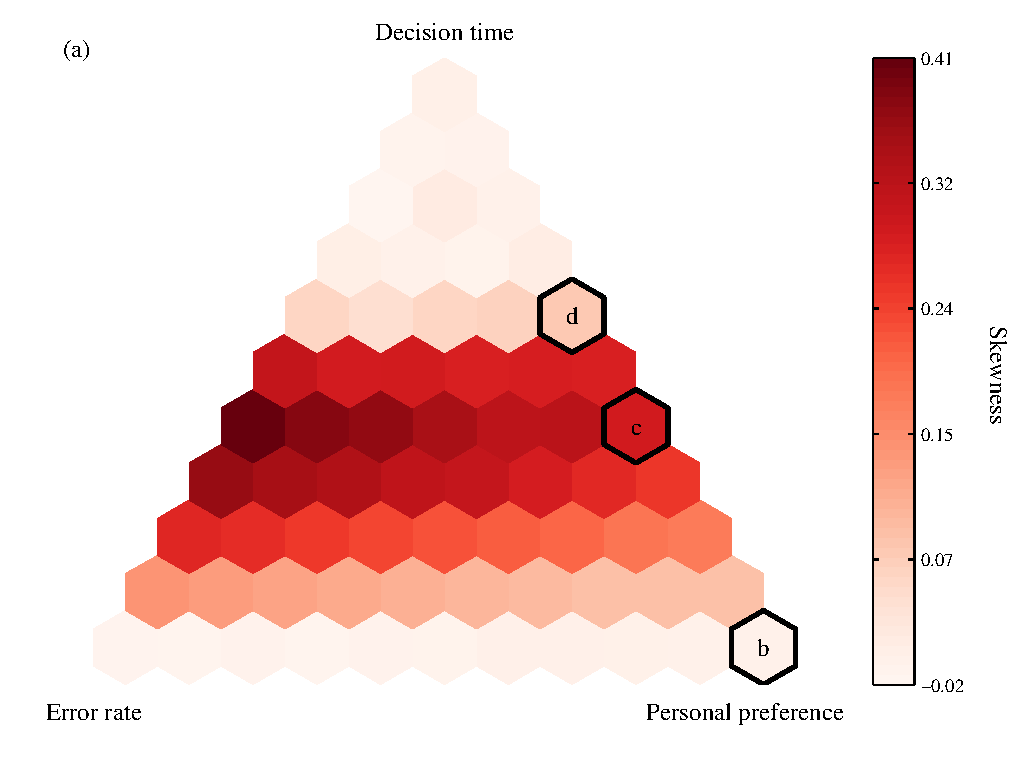
\includegraphics[width=\textwidth]{skewness.pdf}
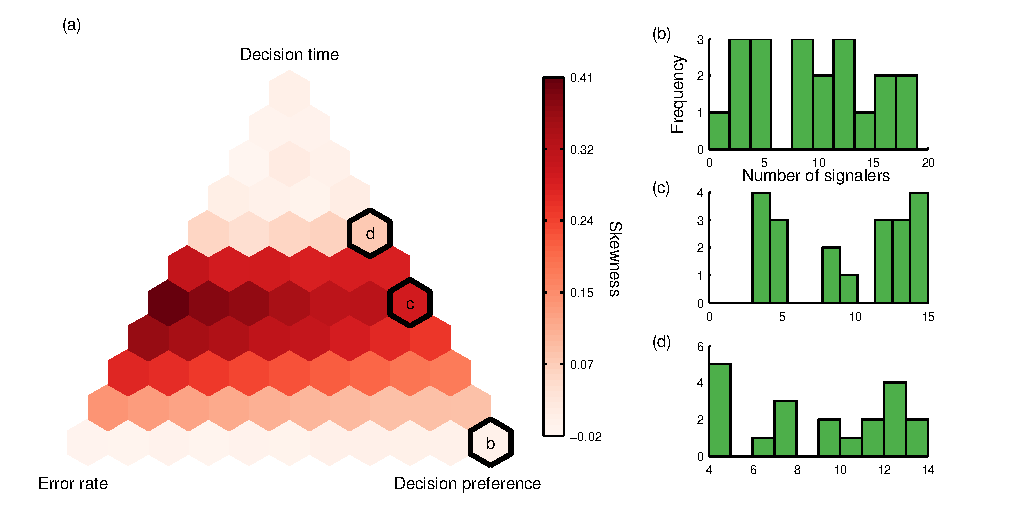
\includegraphics[width=\textwidth]{skewness_histograms.pdf}
\caption{\label{skewness} The average skewness of the distribution of in-degree is maximized at intermediate waiting costs. In the upper panel, the color indicates the average skewness of the distribution of a group using Nash thresholds, as a function of the optimization weights, $w_1$, $w_2$, $w_3$. In the lower left corner of the simplex, only error rate matters ($w_1=1$).  In the upper corner, only decision time matters ($w_2=1$).  In the lower right corner, only preference matters ($w_3=1$). In (b)-(d) we show a histogram for a representative in-degree distribution for a group using the optimization weights as indicated in the simplex with the corresponding letter. Parameters: $w_1=0$, $w_2=0$, $w_3=1$ (c), $w_1=0$, $w_2=0.4$, $w_3=0.6$ (d), $w_1=0$, $w_2=0.6$, $w_3=0.4$ (e),  $N=20$, $b=1$, $r=1$, $\ell=0.1$.}
\end{figure}

\begin{table}[ht]
\centering
\caption{\label{examples}{\bf  Examples of collective computation.} A collective computation can occur when a group of individuals, each of which gathers information and makes a decision in a noisy environment, produces an output that depends in a complex non-linear way on the individuals' decisions. This phenomenon is found in many biological systems. }
\ra{1.3}
\begin{tabular}{@{}lllll@{}}
System & Information & Individual &   Individual decision & Collective computation \\
\cmidrule{1-5} 
brain & moving dots& neural population & to stop firing & decision of the brain
\\  social group & fights won or lost & monkey & to emit a subordination signal & power structure
\\  quorum sensing & signaling molecule & bacteria & to produce signaling molecule & production of toxin
\\ flock movement & environment & bird & where to fly and how quickly & flock movement
\end{tabular}
\end{table}


\begin{table}[ht]
\centering
\caption{\label{variables}{\bf  Variables in the model and their interpretations in neural and social systems.} }
\ra{1.3}
\begin{tabular}{@{}lllll@{}}
Variable & Definition & Neural &   Social \\
\cmidrule{1-4} 
$a$  & value &  degree to which the property  & fighting ability
\\ & & a neural population responds to 
\\ & & is present in the environment&
\\ $b$ & change due to new evidence
\\$c$ & strength of input & coherence of dots & prob. of stronger animal winning
\\ $\ell$ & leak rate
\\ $r$ & interaction rate 
\\ $w_1$ & error rate weight & reward from being ``right" & reward from being ``right"
\\ $w_2$ & decision time weight & penalty for taking a long time & costs of fighting
\\ $w_3$ & prob. of preference weight & ? & benefit from receiving signal
\\ $T_1,T_2$ & decision thresholds
\\$X_1,X_2$ & decision variables &  firing rates of neural populations & opinions about relative dominance
\end{tabular}
\end{table}

%\begin{table}[ht]
%\centering
%\caption{\label{differences}{\bf  Comparison of model in its original application to neural systems and its application to social systems.} Differences are highlighted in red.}
%\ra{1.3}
%\begin{tabular}{@{}lllll@{}}
%&Original neural & & Social \\
%\cmidrule{2-3} \cmidrule{4-4} 
%dimensionality & $1$  && $2$
%\\ group size & $2$ && \fcolorbox{red}{white}{$N$}
%\\decision & difference hits a threshold  && \fcolorbox{red}{white}{one var. hits a threshold}
%\\ optimality criterion &  reward from being ``right" && reward from being ``right"
%\\ & decision time && decision time
%\\ & && \fcolorbox{red}{white}{reward from  receiving signal}
%\\optimization depends on & input strength && input strength
%\\ & noise && noise
%\\ & leak rate && leak rate
%\\ & && \fcolorbox{red}{white}{other animal's threshold}
%\end{tabular}
%\end{table}

\begin{table}[ht]
\centering
\caption{\label{differences}{\bf  Comparison of model in different application.} In its original application to neural systems, the leaky integrator model was reduced to one dimension and the only optimality criteria considered were accuracy and decision time. We study a two-dimensional version of the model and consider the possibility of personal preferences as an additional optimality criterion. This model can be applied to a collection of neural populations in the brain and to a social group of monkeys. Differences between the original neural application and the extended neural and social applications are highlighted in red.}
\ra{1.3}
\begin{tabular}{@{}lllll@{}}
&Original neural & Extended neural & Social \\
\cmidrule{1-3} \cmidrule{4-4} 
decision & difference hits a threshold  & ? & \fcolorbox{red}{white}{one var. hits a threshold}
\\dimensionality & $1$  & $?$ & $2$  
\\ group size & $2$ &\fcolorbox{red}{white}{$N$}& \fcolorbox{red}{white}{$N$}
\\ optimality criterion &  reward from being ``right" & reward from being ``right"& reward from being ``right"
\\ & decision time &decision time & decision time
\\ & &\fcolorbox{red}{white}{reward from  receiving signal} & \fcolorbox{red}{white}{reward from  receiving signal}
\\optimization & no &  \fcolorbox{red}{white}{yes} & \fcolorbox{red}{white}{yes} 
\\ depends on other
\\  individual's threshold
\\ & 
\end{tabular}
\end{table}


\appendix
\section*{Supplementary Information}
\renewcommand{\thesubsection}{\Alph{subsection}.}


\subsection{Derivation of PDEs for waiting time and accuracy \label{pdes_deriv}}

\subsection{Analysis of homogeneous abilities }

\subsection{Supplemental Figures }

\renewcommand{\thefigure}{S\arabic{figure}}
\setcounter{figure}{0}  
\begin{figure}[ht]
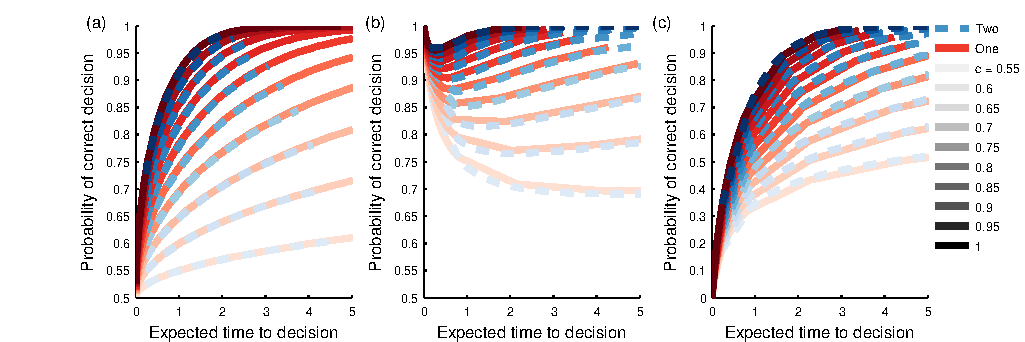
\includegraphics[width=3.415in]{dimensionality_comparison.pdf}

\caption{\label{dimensionality} The accuracy of decision-making is the same for the reduced one-dimensional model and the full two-dimensional model. In each version of the model, changing the decision thresholds changes the probability of a correct decision and the expected time to a decision. Here we show the probability of a correct output as a function of the expected time to a decision, as these thresholds are varied. The red lines correspond to the reduced model and the dashed blue lines correspond to the full model. Decisions of different difficulty ($c$) are represented with lines of different intensity. Parameters: $N=20$, $b=1$, $r=1$, $\ell=0.1$.}
\end{figure}

\begin{figure}[ht]
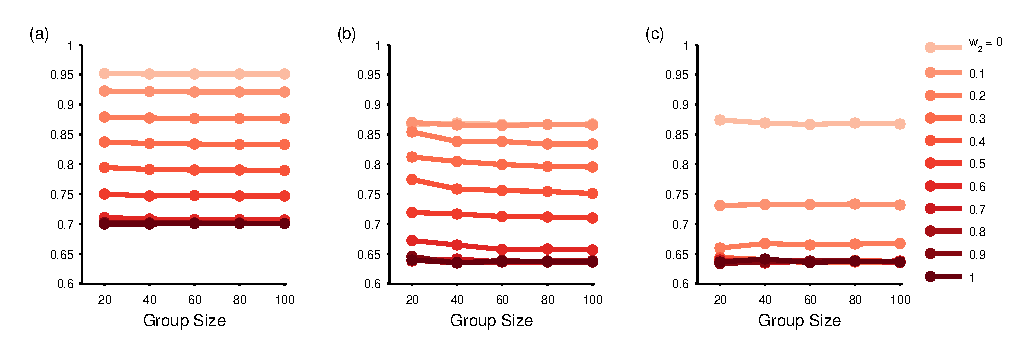
\includegraphics[width=6.83in]{group_size.pdf}
\caption{\label{groupsize} In each panel, group size is on the horizontal axis and average accuracy is on the vertical axis. In (a) we show the average accuracy of the whole group, in (b) we show the average accuracy of the top quartile, and in (c) we show the average accuracy of the bottom quartile. Each line corresponds to a different value of $w_2$. Parameters: $N=20$, $b=1$, $r=1$, $\ell=0.1$, $w_1=0$, $w_3=1-w_2$.}
\end{figure}

\pagebreak
\nocite{*}
\bibliographystyle{plain}
\bibliography{signaling_model}

\end{document}


